\documentclass{article}
\usepackage{tikz}

\begin{document}

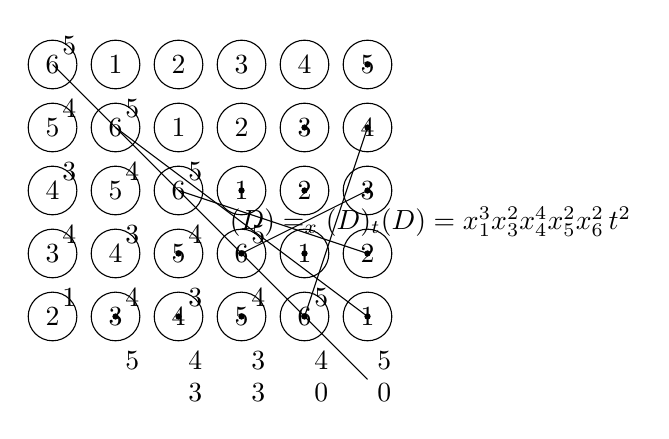
\begin{tikzpicture}[scale=0.8]
    % Define the coordinates for the nodes
    \foreach \i in {1,...,6} {
        \foreach \j in {1,...,5} {
            \pgfmathtruncatemacro{\k}{mod(\i+\j-1, 6)+1}
            \node[circle,draw] at (\i,\j) {\k};
        }
    }
    
    % Draw the lines connecting the nodes
    \draw (1,5) -- (6,0);
    \draw (2,4) -- (6,1);
    \draw (3,3) -- (6,2);
    \draw (4,2) -- (6,3);
    \draw (5,1) -- (6,4);
    
    % Add dots for the empty cells
    \foreach \i in {1,...,6} {
        \foreach \j in {1,...,5} {
            \ifnum\j<\i
                \fill (\i,\j) circle (0.05);
            \fi
        }
    }
    
    % Add labels for the nodes
    \node at (1,5) [above right] {$5$};
    \node at (2,4) [above right] {$5$};
    \node at (3,3) [above right] {$5$};
    \node at (4,2) [above right] {$5$};
    \node at (5,1) [above right] {$5$};
    \node at (6,0) [above right] {$5$};
    \node at (1,4) [above right] {$4$};
    \node at (2,3) [above right] {$4$};
    \node at (3,2) [above right] {$4$};
    \node at (4,1) [above right] {$4$};
    \node at (5,0) [above right] {$4$};
    \node at (1,3) [above right] {$3$};
    \node at (2,2) [above right] {$3$};
    \node at (3,1) [above right] {$3$};
    \node at (4,0) [above right] {$3$};
    \node at (1,2) [above right] {$4$};
    \node at (2,1) [above right] {$4$};
    \node at (3,0) [above right] {$4$};
    \node at (1,1) [above right] {$1$};
    \node at (2,0) [above right] {$5$};
    \node at (3,-0.5) [above right] {$3$};
    \node at (4,-0.5) [above right] {$3$};
    \node at (5,-0.5) [above right] {$0$};
    \node at (6,-0.5) [above right] {$0$};
    
    % Add the weight information
    \node at (7,2.5) {$\wt(D) = \wt_x(D) \wt_t(D) = x_1^3 x_3^2 x_4^4 x_5^2 x_6^2 \, t^2$};
\end{tikzpicture}

\end{document}